% ==============================================================================
% ================================== AUFGABE 1 ================================
% ==============================================================================

\section{Aufgabe 1: 50 Episoden und explorative Datenanalyse}
\label{sec:aufgabe1}

\subsection{Methodik}

Der trainierte \ac{PPO}-Agent wurde deterministisch in einer einzelnen Umgebung über 50 Episoden geführt. Pro Schritt wurden Beobachtung, Aktion, Belohnung, Folgezustand sowie die \texttt{terminated}/\texttt{truncated}-Flags protokolliert, pro Episode wurden Länge und Gesamt-Reward aggregiert. Die Analyse orientiert sich an den in KIPR00 beschriebenen Schritten der Datenexploration \cite[S.~22--23]{2}: deskriptive Statistik, Histogramme, Boxplots, Korrelationsanalyse und Gruppenvergleiche. Ergänzend wird die bei Géron beschriebene Analyse der Aktions- und Entscheidungsstruktur des Agenten herangezogen \cite[S.~970--972]{1}. Die Berechnung der Korrelationskoeffizienten erfolgt nach den in KIPR00 beschriebenen Verfahren (Pearson und Spearman).

\subsection{Ergebnisse}

Über 50 Episoden erzielt der Agent einen mittleren Reward von $281{,}77 \pm 20{,}60$ und eine mittlere Episodenlänge von $226{,}74 \pm 19{,}22$ Schritten (eigene Messung). Die beste Episode (Nr.~33) erzielt $318{,}23$ in $209$ Schritten, die schlechteste (Nr.~48) $247{,}86$ in $234$ Schritten. Alle Episoden enden mit \texttt{terminated=True}, keine läuft in das Zeitlimit. Die Aktionsverteilung zeigt deutlich mehr \emph{noop} (48{,}8\,\%) als \emph{main} (40{,}7\,\%), die Seitenkorrekturdüsen werden mit je rund 5\,\% am seltensten ausgelöst \textit{(eigene Darstellung)}.

\begin{figure}[H]
    \centering
    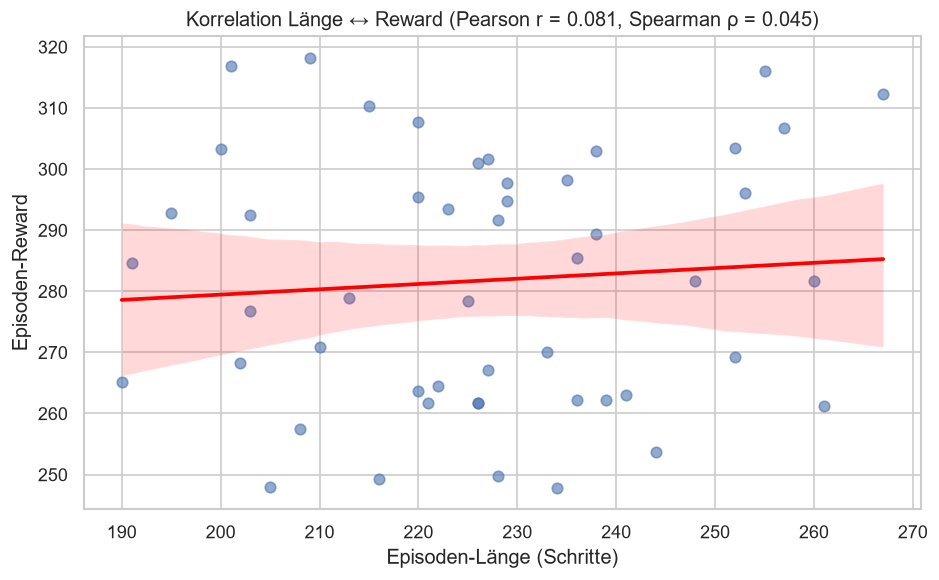
\includegraphics[width=0.8\linewidth]{asset/image/TomaKing_A1_Scatter_Laenge_Reward.png}
    \caption{Korrelation Länge~$\leftrightarrow$~Reward \textit{(eigene Darstellung)}.}
    \label{fig:a1_scatter}
\end{figure}

\begin{figure}[H]
    \centering
    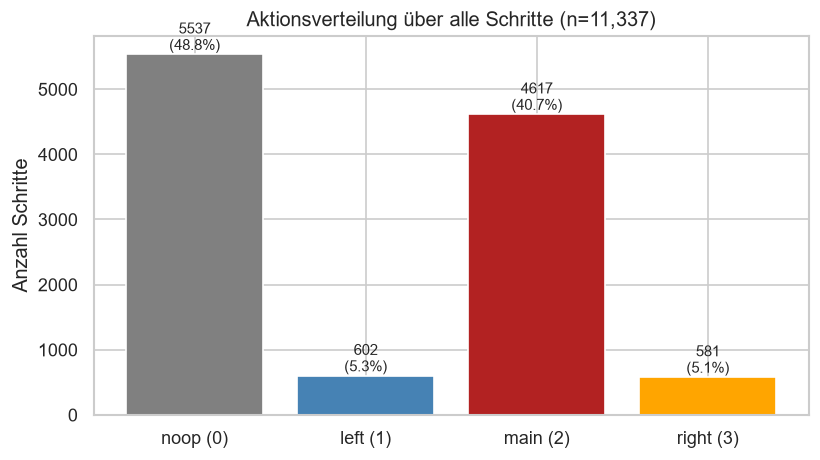
\includegraphics[width=0.8\linewidth]{asset/image/TomaKing_A1_Aktionsverteilung.png}
    \caption{Aktionsverteilung über alle 11\,337 Schritte \textit{(eigene Darstellung)}.}
    \label{fig:a1_actions}
\end{figure}

\begin{figure}[H]
    \centering
    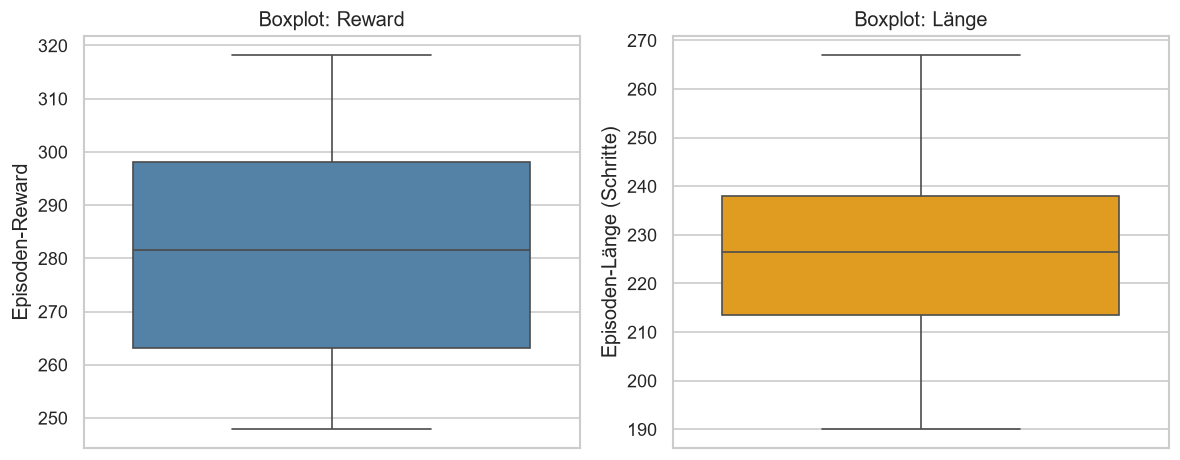
\includegraphics[width=0.65\linewidth]{asset/image/TomaKing_A1_Boxplot_Reward_Laenge.png}
    \caption{Boxplots für Reward und Episodenlänge \textit{(eigene Darstellung)}.}
    \label{fig:a1_box}
\end{figure}

\begin{figure}[H]
    \centering
    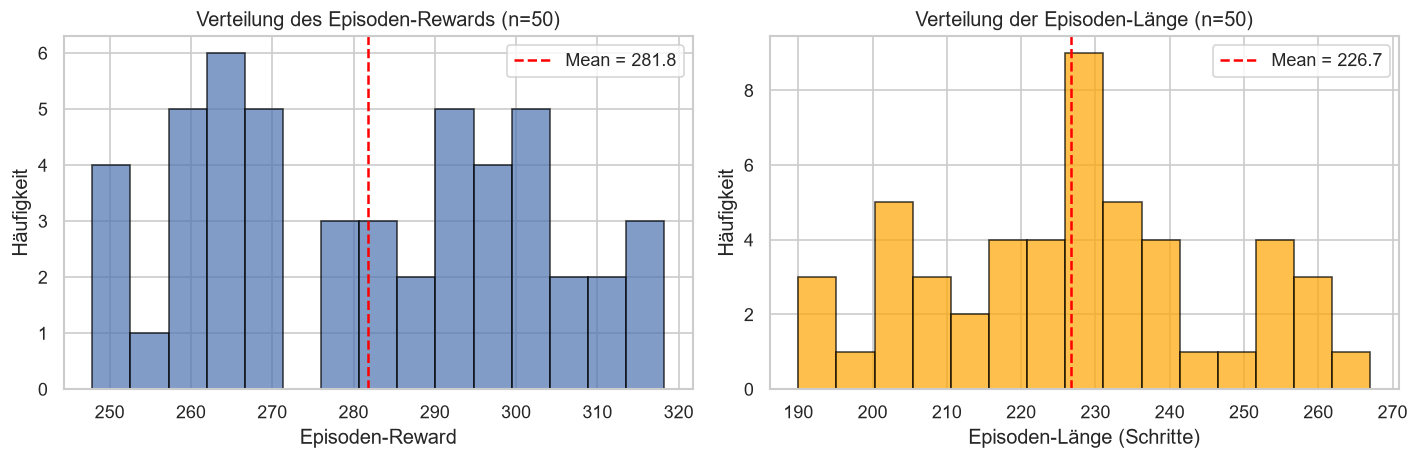
\includegraphics[width=0.7\linewidth]{asset/image/TomaKing_A1_Histogramme_Reward_Laenge.png}
    \caption{Verteilung von Reward und Länge über 50 Episoden \textit{(eigene Darstellung)}.}
    \label{fig:a1_hist}
\end{figure}

\subsection{Interpretation}

Die Pearson-Korrelation zwischen Länge und Reward beträgt $r = 0{,}081$ (Spearman $\rho = 0{,}045$), es besteht praktisch kein linearer oder monotoner Zusammenhang (eigene Berechnung). Dies ist inhaltlich plausibel, weil die Landeprämie ($+100$) unabhängig von der Dauer ist, während jeder Triebwerksschuss Reward kostet. Effiziente, kurze Landungen erzielen daher häufig höhere Rewards als lange, verbrauchsintensive Episoden. Der Befund bestätigt die in KIPR00 betonte Notwendigkeit, Korrelationen fachlich zu interpretieren und nicht als Kausalaussage zu lesen \cite[S.~23]{2}. Die visuelle Inspektion der Verteilungen (Abbildung~\ref{fig:a1_hist} und Abbildung~\ref{fig:a1_box}) stützt diese Einschätzung.

% ==============================================================================
% ================================== AUFGABE 1 ================================
% ==============================================================================